%\newcommand{\Exp}{\mathbb{E}}

% reset section counter
\setcounter{section}{0}

%\metadata{lecture ID}{Your names}{date}
\metadata{3}{Luis Alcaraz}{April 16, 2021}

\sec{Review and overview}

	In the previous lecture, we covered bias-variance trade-off, local linear regression and had a brief introduction to linear smoothers. 
	
	In this lecture we will continue exploring classical non-parametric methods. First, by exploring local polynomial regression as an extension of local linear regression. Then, different methods of optimizing regression are evaluated, including cross validation where one selects various hyperparameters and dropout methods where the data set is split into validation and training sets. Finally, the rest of the lecture covered splines as a new framework for an non-parametric algorithm. 
	
\sec{Local polynomial regression}
As we saw in the previous lecture, local linear regression as in Fig.~\ref{fig:local_linear_regression example} extends local averaging, where local averaging fits a locally constant function while local linear regression fits a linear one, fixing the design bias locally. To fix the tension within local linear regression, we now apply local polynomial regression, which just like local linear regression extends local averaging, local polynomial extends local linear regression.

Essentially, in local polynomial regression, we are fitting polynomial functions locally. We first start by fixing $x$.

\begin{figure}[htbp!]
        \begin{center}
        \begin{tikzpicture}
            \begin{axis}[
            axis lines=middle,
            xtick=\empty, ytick=\empty,
            xlabel=$x$,ylabel=$y$,
            ]
	            \addplot[
		            thick,
		            blue,
	                ] table [y index=1, x index=0, col sep=comma]{figure/Lecture03/statsdata.txt};
                \addplot [only marks, mark = o, thick, red] table [y index=1, x index=0, col sep=comma]{figure/Lecture03/statsdata.txt};
               
                
                \addlegendentry{$r(x)$}
                \addlegendentry{$(x_i, Y_i)$'s}
	        \end{axis}
        \end{tikzpicture}
        \caption{Graphical representation of local linear regression (LLR).}
        \label{fig:local_linear_regression example}
        \end{center}
        \end{figure}





Once we have a fixed $x$, we now want to approximate the function $r(\cdot)$ in the neighborhood of $x$ by defining the function $P_x(u;a)$ with $a = (a_0, \cdots, a_p)$ where\footnote{$p!$ is a convenient choice if we want to take $k$-th order derivative of $P_x(u,a)$ at $u=x$, i.e. $\left.\frac{\mathrm d^k}{\mathrm d u^k}P_x(u,a)\right|_{u=x} = a_k$ for all $k=0,\cdots, p$.} 
\begin{align}
P_x(u;a) = a_0 + a_1(u - x) + \frac{a_2}{2}(u - x)^2 + ... + \frac{a_p}{p!}(u - x)^p  
\end{align}
 With this new approximate $P_x$, we now want to fit this degree-$p$ polynomial to the data around point $x$. Much like the logic with local linear regression, we are no longer assuming $r(x)$ is neither constant or locally linear, but rather we assume $r(x)$ is a polynomial function locally. Therefore, we minimize over $a$, giving us the minimized equation: 

\begin{align}
    \hat{a} = (\hat{a}_0, ..., \hat{a}_p) &= \argmin_{(a_0,..., a_p) \in \R^{p+1}} \sum_{j=1}^{n}w_j(Y_j - P_x(u_j;a))^2 \nonumber \\
    &= \argmin_{(a_0,..., a_p) \in \R^{p+1}} \sum_{j=1}^{n}w_j\left(Y_j - (a_0 + a_1(u - x) + ... + \frac{a_p}{p!}(u - x)^p)\right)^2,
  \end{align}
where $w_j = K \left(\frac{x-x_j}{h}\right)$ for some kernel function $K$. Notice that we can rewrite this equation into
\begin{align*}
\argmin_{a \in \R^{p+1}} \sum_{j=1}^{n}w_j(Y_j - a^\top z_j)^2, 
\end{align*}
where $a$ and $z_j$ are
\begin{align*}
a = \begin{bmatrix} a_0 \\ \vdots \\a_p \end{bmatrix}, \qquad
z_j = \begin{bmatrix} 1 \\ x_j-x \\ \vdots \\\frac{1}{p!}(x_j-x)^p \end{bmatrix}.
\end{align*}
As we can see, this function closely resembles local linear regression with the exception of $P_x$ representing degree-$p$ polynomials. Therefore, we can classify it as weighted linear regression with vector $a$ as parameter and $z_j$'s as the input, giving us a very similar final estimator function to local linear regression
\[
\hat{r}(x) = P_x(x;\hat{a}) = \hat{a}_0.
\]
It is noted when using local polynomial regression, the convention is to use up to degree 3 polynomials as higher-degree polynomials are not much helper in complex data sets. Also note, local polynomial regression is also a linear smoother.
\sec{Cross validation}
There are different forms of cross validation that can be conducted on an algorithm. The main reason to the use of cross validation is reducing the chance of over-fitting through altering various hyperparameters. This cross-validation technique is widely used in machine learning, specifically, neural nets, when trying to create models that best fit specific datasets. Nevertheless, in our case, we will be looking at cross validation for local polynomial regression which concerns selecting the optimal bandwidth $h$, degree polynomial $p$, and which method (like splines, regressogram, etc.) is used. The reason we care about cross validation is in order to optimize our model, and therefore our results. Recall we want to evaluate and minimize 
\begin{align*}
\mathrm{MSE} &= \E_{Y_i} \left[\mathrm{MSE}(\hat r)\right] \nonumber \\
& =  \E \left[\frac{1}{n}\sum_{i=1}^{n}(\hat{r}(x_i) - r(x_i))^2\right] ,
\end{align*}
where
 \[
\mathrm{MSE}(\hat r) = \frac{1}{n}\sum_{i=1}^{n}(\hat{r}(x_i) - r(x_i))^2.
\]
As we have seen before, this issue cannot simply be solved with minimizing the training error
\[
\frac{1}{n} \sum_{i = 1}^{n} (Y_i - \hat{r}(x_i))^2,
\]
as setting $h=0$ gives zero training error, as $\hat{r}(x_i) = Y_i$
\subsec{Holdout dataset}
One method of cross validation that is widely used in machine learning is holdout set. However, this is only useful when you have a large dataset, something rarely available in non-parametric statistics. Nevertheless, holdout is a technique where a dataset is split into two sets where you take a random permutation of $1,\cdots, n$ as $i_1,...,i_n$, such that you use $(X_{i_1}, Y_{i_1}),..., (X_{i_m}, Y_{i_m})$ for training and $(X_{i_{m+1}}, Y_{i_{m+1}}),..., (X_{i_n}, Y_{i_n})$ as a validation set.
\subsec{Leave-one-out estimate}
Another technique for cross validation is leave-one-out estimate where you have an estimator for the risk
\[
\hat{R}(h) = \frac{1}{n} \sum_{i = 1}^{n}(Y_i - \hat{r}_{-i}(x_i))^2,
\]
where $\hat{r}_{-i}(\cdot)$ is the estimator applied to the dataset excluding $x_i$. So basically you remove $x_i$ from the dataset, and then apply the estimator, and finally use estimator on $x_i$ to see if it can produce $Y_i$ with relative small error. To implement this, recall a general linear smoother can be written as
\[
\hat{r}(x) = \sum_{j = 1}^{n} l_j(x) Y_j, \quad \sum_{j=1}^n l_j(x) = 1.
\]
Therefore, for the leave-one-out estimator, we can obtain that
\begin{align*}
    \hat{r}_{-1}(x) = \sum_{j \not = i} \left( \frac{ l_j(x) }{\sum_{j \not = i} l_j(x)} \cdot Y_j \right).
  \end{align*}
For the kernel estimator, $\hat{r}_{-1}(x)$ defined in the equation above is indeed the estimator applied on $(X_{1}, Y_{1}),..., (X_{n}, Y_{n})$ excluding $(X_{i}, Y_{i})$. Here $\hat{R}$ is almost an unbiased estimator for the predictive risk. Now follows the question on how to computer $\hat{R}$ efficiently. We will do this in the form of a theorem.
\begin{theorem}
	If $\hat{r}$ is a linear smoother \[
	\hat{r}(x) = \sum_{j =1}^{n} l_j(x) Y_j,
	\]
	then
	\begin{align}
	\hat{R}(h) = \frac{1}{n}\sum_{i=1}^{n} \frac{(Y_i - \hat{r}(x_i))^2}{1 - L_{ii}},
	\end{align}
	where $L_{ii} = l_i(x_i)$. 
\end{theorem}
\begin{proof} Consider the estimator \[
\hat{r}_{-1}(x_i) = \frac{\sum_{j \not = i} l_j(x_i) Y_j}{\sum_{j \not = i} l_j(x_i)},
\] 
Recall the sum of the weights for data point $x$ is always $1$, therefore we can rewrite the estimator as
\begin{align*}
    \hat{r}_{-1}(x_i) &= \frac{\sum_{j = 1}^{n} l_j(x_i) Y_j - l_i(x_i)}{\sum_{j \not = i} l_j} \\
    &= \frac{\hat{r}(x_i) - l_i(x_i)Y_i}{1 - L_{ii}}. \\
  \end{align*}
  Therefore,
  \begin{align*}
    \hat{R}(h) &= \frac{1}{n} \sum_{i = 1}^{n}(Y_i - \hat{r}_{-i}(x_i))^2\\
    &= \frac{1}{n} \sum_{i = 1}^{n}\left(Y_i - \frac{\hat{r}(x_i) - l_i(x_i)Y_i}{1 - L_{ii}}\right)^2\\
    &= \frac{1}{n} \sum_{i = 1}^{n}\left(\frac{Y_i - \hat{r}(x_i)}{1 - L_{ii}}\right)^2,
  \end{align*}
  as desired. 
\end{proof}

\sec{Splines}
\subsec{Penalized Regression}
To motivate the use of splines, first let us recall the MSE for local linear regression where we seek to minimize $\int r''(x)^2dx$. In the case where we explicitly leverage the smoothest function that fits the data is known as penalized regression. We can rewrite the function as
\[
\argmin_{\hat{r}} \sum_{i =1}^{n} (Y_i - \hat{r}(x_i))^2 + \lambda J(\hat{r}) \triangleq L_\lambda(\hat{r}).
\]
where $J(\hat{r}) = \int r''(x)^2dx$. Let us consider one of the extreme cases when
\begin{figure}[htbp!]
        \begin{center}
        \begin{tikzpicture}
            \begin{axis}[
            legend pos=south east,
            axis lines=middle,
            xtick=\empty, ytick=\empty,
            xlabel=$x$,ylabel=$y$,
            ymin=-5
            ]
	            \addplot[
		            thick,
		            blue,
	                ] table [y index=1, x index=0, col sep=comma]{figure/Lecture03/statsdata.txt};
                \addplot [only marks, mark = o, thick, red] table [y index=1, x index=0, col sep=comma]{figure/Lecture03/statsdata.txt};
                \addplot[
                domain = 0:7,
		            thick,
		            red,
	                ] {-(cos(10*pi * deg(x-4)) + .5 * (x-4)^2) + 6};
               
                
                \addlegendentry{$r(x)$}
                \addlegendentry{$(x_i, Y_i)$'s}
                \addlegendentry{$\lambda = \infty$}
	        \end{axis}
        \end{tikzpicture}
        \caption{Example of extreme cases when $\lambda = \infty$.}
        \label{fig:regression example}
        \end{center}
        \end{figure}
$\lambda = \infty$. In this case, $J(\hat{r})$ can only be zero since $r''(x) = 0$ and $\hat{r}$ can only be linear. Here, what spline is doing is that you do not have to be so strict with being linear, in addition to controlling second order derivatives. We can now move onto defining splines.
\subsec{Splines}
Splines themselves are family of functions $f$, where we have the set points $\xi_1 < \xi_2 < ... , \xi_k$ (also known as knots) contained in some interval $[a,b]$. Generally, $M$-th order splines are piecewise $(M-1)$-degree polynomial with continuous $(M-2)$-th order derivatives at the knots. More specifically, a cubic spline ($4$-th order spline) $q$ is a continuous function such that
\begin{itemize}
    \item $q$ is a cubic polynomial on $(a, \xi_1]$,$ [\xi_1, \xi_2]$, ..., $[\xi_k-1, \xi_k]$, $[\xi_k, b)$, where you have fixed cubic polynomial between $\xi_i$ and $\xi_{i+1}$. 
    \item $q$ has continuous first and second derivatives at the knots.
\end{itemize}

However, there is another type of spline, known as a natural spline. This spline is one that extrapolates linearly beyond the boundary knots. After defining a few of these notions, we can intuitively see piecewise polynomials has relative smoothness properties and will allow us to arrive to a solution for the penalized objective. We will now prove a theorem that demonstrates this. 
\subsec{Background: subspaces}
        A subspace is a set of functions $f$ which form a subspace $\mathcal{F}$  if $\forall f,g \in \mathcal{F}$, $\lambda_1f_1 + \lambda_2g \in \mathcal{F}$ for all $\lambda_1, \lambda_2 \in \R$.
        Furthermore, a subspace of functions has dimension of at most $k$ if $\exists f_1, ...,f_k \in \mathcal{F}$ such that $\forall f \in \mathcal{F}$, $f$ can be represented as \[
        f = \sum_{i = 1}^{k}\lambda_if_i
        \]
        for some $\lambda_1, \cdots, \lambda_k \in \R$.  Note $f_i$'s are often refereed to as basis.
\begin{theorem} The function that minimizes $L_{\lambda}(\hat{r})$ is a natural cubic spline with knots at the data points. The minimizer has to be a cubic spline. 
\end{theorem}
Therefore, the minimizer of the penalized objective has an estimator that is called a smoothing spline. Note that the search space in this case is dramatically reduced, because the number of natural cubic splines than the number of all functions. Furthermore, to have the smoothest function, you do not need any higher-order derivatives beyond the third order. To prove this let us consider the following lemma.
\begin{lemma} All cubic splines with knots $\xi_1,...,\xi_k$ form a $(k+4)$-dimensional subspace of functions. Specifically, there exists some $h_1. ..., h_{k+4}$ such that every cubic spline $f$ can be represented as 
	\begin{align*}
		f = \sum_{i=1}^{k+4}\lambda_i h_i,
	\end{align*}
where the $\lambda_i$'s serve as parameters. 
\end{lemma}

\begin{proof}
	Let us consider the case where we have $f,g$ being cubic splices with fixed knots $\xi_1,...,\xi_k$. Therefore, $f+g$ is also a cubic splice. Now we will show why the space of cubic splines with fixed knots also form a $(k+4)$-dimensional subspace. Notice that a cubic spline can be represented as \[
	q(x) = a_{3,i}x^3 + a_{2,i}x^2 + a_{1,i}x + a_{0,i}
	\]
	For all $x \in [\xi_i, \xi_{i+1}]$ where $\forall i = 0, ..., k$. The convention for knot assignment is: $\xi_0 = a$, $\xi_{k+1} = b$, in addition to the convention of $a,b$ equating to ($-\infty,\infty$). However, note that $a_{t,i}$'s have to satisfy constraints pertaining to the $(M-2)$-th order derivation requirements explored earlier. To prove the lemma, consider the following functions
	\begin{align*}
	h_1(x) & = 1, \\
	h_2(x) & = x, \\
	h_3(x) & = x^2, \\
	h_4(x) &= x^3, \\
	h_{i+4}(x) &= (x-\xi_i)_+^3, \quad i =1, \cdots, k.
	\end{align*}
	where $t_+$ is the ReLU function utilized throughout machine learning $\max\{t,0\}$. We prove that they are the desired basis by induction.  When there is no knots, a degree 3 polynomial can be represented by combinations of $h_0, h_1, h_2, h_3$. 
	
	Suppose the inductive hypothesis holds true for $k-1$ knots. We can take the spline $\widetilde{q}(x)$ which spans over $\xi_1,...,\xi_{k-1}$ where we define $\widetilde{q}(x) = q(x)$ for all $x \in [\xi_{k-1},\xi_k]$. Suppose \[
	q(x) =  a_{3,k-1}x^3 + a_{2,k-1}x^2 + a_{1,k-1}x + a_{0,k-1}
	\]
	on $[\xi_{k-1}, \xi_k]$. For $\widetilde{q}(x)$ on $[\xi_k,b)$: \[
	\widetilde{q}(x) =  a_{3,k-1}x^3 + a_{2,k-1}x^2 + a_{1,k-1}x + a_{0,k-1}
	\] Since we also know that $\widetilde{q}$ is a cubic spline with $k-1$ knots, by the inductive hypothesis \[
	\widetilde{q}(x) = \sum_{i=1}^{k+3}\lambda_ih_i(x).
	\]
	Therefore, we can deduce that for all $x \leq \xi_k$ $q(x) - \widetilde{q}(x)$ is zero, while for [$\xi_k,b$) is a degree 3 polynomial. 
	\begin{figure}[!hb]
		\begin{center}
			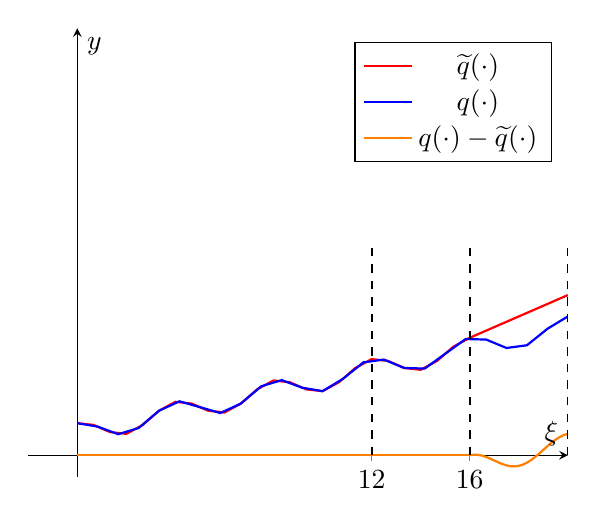
\begin{tikzpicture}
				\begin{axis}[
					legend pos=north east,
					axis lines=middle,
					xtick={16,12}, ytick=\empty,
					xmin=-2, xmax=20,
					ymin=-2, ymax=40,
					xlabel=$\xi$,ylabel=$y$,
					]
					\addplot[
					domain = 0:16,
					thick,
					red,
					] {cos(.5 * pi * deg(x)) + .5*x + 2};
					\addplot[
					domain = 0:20,
					thick,
					blue,
					] {cos(.5 * pi * deg(x)) + .5*x + 2};
					\addplot[
					domain = 16:20,
					thick,
					orange,
					] {cos(.5 * pi * deg(x)) + .5*x - 9};
					\addplot[
					domain = 0:16,
					thick,
					orange,
					] {0};
					\addplot[
					domain = 16:20,
					thick,
					red,
					] {x - 5};
					
					\addplot[thick, samples=50, dashed,black] coordinates {(12,0)(12,20)};
					\addplot[thick, samples=50, dashed,black] coordinates {(16,0)(16,20)};
					\addplot[thick, samples=50, dashed,black] coordinates {(20,0)(20,20)};
					
					
					\addlegendentry{$\widetilde{q}(\cdot)$}
					\addlegendentry{$q(\cdot)$}
					\addlegendentry{$q(\cdot) - \widetilde{q}(\cdot)$}
					
				\end{axis}
			\end{tikzpicture}
			\caption{$q(\cdot) - \widetilde{q}(\cdot)$, $12= \xi_{k-1}$, $16 = \xi_k$}
			\label{fig:regression example}
		\end{center}
	\end{figure}
	\\Furthermore, recall that we know that $q(x)$ and $\widetilde{q}(x)$ have continuous derivatives. Notice that
	\[
	q(\xi_k) - \widetilde{q}(\xi_k) = 0 = b_0,
	\] \[
	q'(\xi_k) - \widetilde{q}'(\xi_k) = 0 = b_1, 
	\] \[
	q''(\xi_k) - \widetilde{q}''(\xi_k) = 0 = 2b_2.
	\]
	And given we can rewrite $q(x) - \widetilde{q}(x) = b_3(x-\xi_k)^3 + b_2(x-\xi_k)^2 + b_1(x-\xi_k) + b_0$. Therefore, $q(x) - \widetilde{q}(x) = b_3(x - \xi_k)^3$ for all $x \geq \xi_k$. Rewriting it shows $q(x) - \widetilde{q}(x) = b_3(x - \xi_k)^3$ and hence
	\begin{align*}
		q(x) &= \widetilde{q}(x) + b_3(x - \xi_k)_+^3 = \sum_{i=1}^{k+4}\lambda_ih_i(x).
	\end{align*}
	where $\lambda_{k+4} = b_3$
\end{proof} 
	Given this lemma, we will now show that degree $3$ spline $g$ is the minimizer of $L_\lambda(\hat{r})$. To do this, we will construct a natural spline that matches $g$ on $x_1, ..., x_n$, namely $\widetilde{g}$, where we define $\widetilde{g}(x) = g(x)$ for all $x \in \left\{x_1, \cdots, x_n\right\}$. This implies \[
	\sum_{i =1}^{k}(Y_i - g(x_i))^2 = \sum_{i =1}^{k}(Y_i - \widetilde{g}(x_i))^2  
	\]
	Next we will show that $\int \widetilde{g}''(x)^2dx \leq \int g''(x)^2dx$ which will then indicate that $L_\lambda(\widetilde{g}) \leq L_\lambda(g)$. Notice that in these two inequalities, equality is attained at $g = \widetilde{g}$.
	Let us consider $h$ where $h = g - \widetilde{g} $. Given this, we only need to deduce $h(x) = 0$. Note that 
	\begin{align*}
		\int \widetilde{g}''(x)^2dx &= \int (\widetilde{g}''(x) + h''(x))^2dx \\
		&= \int (\widetilde{g}''(x))^2dx + 2\int \widetilde{g}''(x) h''(x)dx + \int (h''(x))^2dx \\
		&\geq \int (\widetilde{g}''(x))^2dx + 2\int \widetilde{g}''(x) h''(x)dx
	\end{align*}
	Here we want to show that $2\int \widetilde{g}''(x) h''(x)dx = 0$. By integration by parts, we can show: 
	\begin{align*}
		\int_{a}^{b} \widetilde{g}''(x) h''(x)dx &= \left.\widetilde{g}(x)''h'(x) \right|_{a}^b - \int_{a}^{b} h'(x)\widetilde{g}'''(x)dx.
	\end{align*}
	Recall that in natural splice, $\widetilde{g}'' = 0$, therefore $\widetilde{g}''(a) = 0$ and $\widetilde{g}''(b) = 0$, leaving us with
	\begin{align*}
		\int_{a}^{b} \widetilde{g}''(x) h''(x)dx &= - \int_{a}^{b} h'(x)\widetilde{g}'''(x)dx.
	\end{align*}
	Here, we can identify $\widetilde{g}''(x)$ as constant $c_i$ on $[\xi_i, \xi_{i+1}]$ given that $\widetilde{g}$ is a degree-$3$ polynomial on the interval. This allows us to further expand 
	\begin{align*}
		\int_{a}^{b} \widetilde{g}''(x) h''(x)dx &= - \int_{a}^{b} h'(x)\widetilde{g}'''(x)dx \\
		&= - \int_{a}^{x_1} h'(x)\widetilde{g}'''(x)dx  - \sum_{i = 1}^{n-1}\int_{x_i}^{x_{i+1}} h'(x)\widetilde{g}'''(x)dx - \int_{x_n}^{b} h'(x)\widetilde{g}'''(x)dx \\ 
		&= -c_0 \int_{a}^{x_i} h'(x)dx  - \sum_{i = 1}^{n-1} c_i\int_{x_i}^{x_{i+1}} h'(x)dx - c_{n} \int_{x_n}^{b} h'(x)dx.
	\end{align*}
	Here, $c_0$ and $c_n$ are zeros because $\widetilde{g}$ is linear near the boundary given that it is a natural spline, leaving us with
	\begin{align*}
		\int_{a}^{b} \widetilde{g}''(x) h''(x)dx &=  - \sum_{i = 1}^{n-1} c_i\int_{x_i}^{x_{i+1}} (h'(x))dx \\ 
		&=   - \sum_{i = 1}^{n-1} c_i (h(x_{i+1}) - h(x_i))dx  \\
		& = 0,
	\end{align*}
	where the last line follows since $g = \widetilde{g}$ on knots, $h(x_{i+1})$ and $h(x_{i})$ are zero. 


%\subsection{}